\documentclass{article}
\usepackage[english]{babel}
\usepackage[utf8]{inputenc}
\usepackage[parfill]{parskip}
\usepackage{amsmath,amssymb,amsthm}
\usepackage{a4wide}
\usepackage{color}
\usepackage{graphicx}
\usepackage{booktabs}
\usepackage{tikz}
\usepackage{pgfplots}
\pgfplotsset{compat=newest}
\usetikzlibrary{calc}
\newcommand{\eps}{\varepsilon}
\newcommand{\bigo}[1]{\mathcal{O}\left(#1\right)}
\newcommand{\note}[1]{\emph{\color{blue}#1}}
\renewcommand{\L}{\mathcal{ L}}
\newcommand{\R}{\mathbb{ R}}
\newcommand{\N}{\mathbb{ N}}
\newtheorem{defin}{Definition}

\newcommand{\macromesh}{\mathcal{ B}_H}
\newcommand{\micromesh}{\mathcal{ K}_h}
%\renewcommand{\L}{\mathcal{ L}}
\newcommand{\boundaryz}{\partial Z}
\renewcommand{\H}{\mathcal{ H}}
\newcommand{\B}{\mathcal{ B}}
\newcommand{\dealii}{deal.ii{}}
\renewcommand{\P}{\mathbb{ P}}
\newcommand{\K}{\mathcal{ K}}
\newcommand{\V}{\mathcal{ V}}
\newcommand{\embed}{\hookrightarrow}
\renewcommand{\div}{\operatorname{div}}
\renewcommand{\vec}{\mathbf}
\newtheorem{lem}{Lemma}
\newtheorem{prop}{Proposition}
\newtheorem{thm}{Theorem}
\newtheorem{assumption}{Assumption}
\title{Multiscale deal.II implementation for an elliptic-elliptic system with macroscopically-dependent microscopic pull-back operators}
\author{Omar Richardson}

\begin{document}
\maketitle

\section{Introduction}
This report contains a summary on the activities during a five week-research visit to the MPS in the University of Sussex, where Omar Richardson collaborated with Omar Lakkis and Chandrasekhar Venkataraman, and the subsequent continuation in Karlstad.

This report is structured as follows. Section~\ref{sec:problem} describes the problem under consideration.
Section~\ref{sec:wellposedness} describes how the weak formulation is discretized, as well as how the domain mapping is defined.
Section~\ref{sec:dealii} contains details on the implementation of the PDE system.
In Section~\ref{sec:manufactured}, we describe the formulation of a toy problem that we use to benchmark the implementation, as well as the issues that arise.
Finally, Section~\ref{sec:next} describes the future steps in this project.

\section{Problem description}
\label{sec:problem}
The following problem is posed on two scales; let $\Omega \subset \R^{d_1}$ be the macroscopic domain and $Y \subset R^{d_2}$ be a microscopic domain with $d_1,d_2 \in \{1,2,3\}$. Furthermore, let us for each $x \in \Omega$ define a microscopic domain $Y_x \subset Y$.
This allows us to define the composite (multiscale) domain $\Lambda$ as
\begin{equation*}
    \Lambda := \bigcup_{x\in\Omega} \left(  \{ x \} \times Y_x\right)
\end{equation*}
Let $\zeta \in C(\bar{\Omega};C^{1-}(\bar{Z},\bar{Y}))$ be a mapping. Then, each of the microscopic domains $Y_x$ is constructed from a base domain $Z$ as follows:
\begin{equation}
    \zeta(x,Z) = Y_x.
\end{equation}
Furthermore, assume that $\zeta(x,\cdot)$ is invertible for each $x$ and that
\begin{equation}
    c_*  \leq \mathrm{det}\nabla_y \zeta(x,\cdot) \leq c^*,
\end{equation}
where $\nabla_x$ represents Clarke's generalized gradient, and that
\begin{equation}
    \zeta^{-1}(x,\cdot):  C(\bar{\Omega};C^{1-}(\bar{Y},\bar{Z})).
\end{equation}
More details about this setup are present in \cite{sebamPhD} or \cite{lakkis13}.

The problem can be formulated as follows: Find  $ \tilde{u}: \Omega \to \R $ and $v: \Lambda\to \R$ that satisfy:

\begin{align}
    \label{eq:main_macro}&\div_x\left( -D_1(x) \nabla_x \tilde{u}(x))\right) = \int_{Y_x} v(x,y) dy + f(x),&x \in \Omega \\
    \label{eq:main_micro}&- D_2 \Delta_y v(x,y) = g(x,y,\tilde{u}(x) - u^D(x)),&  x\in \Omega, y \in Y_x \\
    \label{eq:main_macro_bc}&\tilde{u}(x) = u^D(x), & x\in \partial \Omega,y \in Y_x\\
    \label{eq:main_micro_bc}& - D_2 \nabla_y v(x,y) \cdot n = \kappa(v(x,y) - p(x,y)), &x\in \Omega, y \in \Gamma_x
\end{align}
where  $g: \Lambda \times \R \to \R$ and $f:\Lambda \to \R$ are given functions. We refer to \eqref{eq:main_macro}-\eqref{eq:main_micro_bc} as ($P_1$).

\subsection{Weak solutions}

We are interested in solutions to ($P_1$) in the weak sense. This is motivated by the fact that the underlying structured media can be of composite type, allowing for discontinuities in the model parameters.

We use $V$ and $W$ to denote the following function spaces:
\begin{align*}
    V &:= H^1_0(\Omega)\\
    W &:= L^2 \left( \Omega; H^1(Y_x)\right)
\end{align*}
Let us for the rest of this discussion use the notation $u := \tilde{u} - u^D$.

\begin{defin}[Weak solution]
    A weak solution of ($P_1$) is a pair
    \begin{equation*}
        (u,v)\in V\times W
    \end{equation*}
    that satisfies for all test functions $(\varphi,\psi) \in V\times W$ the identities
\begin{equation}
    \begin{split}
        &\int_\Omega D_1(x) \nabla_x u \cdot \nabla_x \phi dx = \int_\Omega \left( \int_{Y_x} vdy + f \right)\phi dx + \int_\Omega \div_x \left(D_1(x)\nabla u^D(x) \right)
    \end{split}
    \label{eq:weak_macro}
\end{equation}
and
\begin{equation}
    \label{eq:weak_micro}
    \int_\Omega\int_{Y_x} D_2 \nabla_y v \cdot \nabla_y \psi dy dx + \int_\Omega\int_\Gamma \kappa (v - p) \psi d\sigma_y dx
     =\int_\Omega \int_{Y_x} g(u) \psi dy dx
\end{equation}
\end{defin}

\section{Space discretization}
\label{sec:wellposedness}
In this section we pose the finite element approximation of the weak solution of ($P_1$).
First, we introduce the necessary tools for defining the Galerkin approximation.

We use one mesh partition for each of the two spatial scales. Subsequently, we ensure that each microscopic finite element space follows from a base space through mapping $\zeta$.
Let $\B_H$ be a mesh partition for $\Omega$ consisting of simplices. We denote the diameter of an element $B \in \B_H$ with $H_B$, and the global mesh size with $H:= \max_{B \in \B_H} H_B$.
We introduce a similar mesh partition $\K_h$ for $Z$ with global mesh size $h:= \max_{K \in \K_h} h_K$.

Let $\mathcal{N}_1$ denote the set of degrees of freedom in $\macromesh$. For each $i \in \mathcal{N}_1$, we define a microscopic finite element space $W_h^i$ with $\mathcal{N}_2$ degrees of freedom, located in $x_i$.

The macroscopic and microscopic finite element spaces $V_H$ and $W_h^i$ are then defined as, respectively:
\begin{align*}
    V_H &:= \left\{ \left. v \in C^0(\bar{\Omega})\right|\,v|_B \in \P^l(B) \mbox{ for all } B \in \B_H, v=0 \in \partial \Omega  \right\},\\
        W_h^i &:= \left\{ \left. w \in C^0(\bar{Y}_{x_i})\right|\,w|_K \circ \zeta^{-1} \in \P^l(K) \mbox{ for all } K \in \K_h  \right\}.
\end{align*}
where $\P^k(W)$ denotes the function space of polynomials of degree $k$ on set $W$.
Finally, let $W^0_h$ be defined as the finite element space on reference domain $Z$.

Let $\langle \xi_B \rangle_{\B_H}:= \operatorname{span}(V_H)$ and $ \langle \eta_K \rangle_{\K_h}:= \operatorname{span}(W_h)$ defined such that
\begin{equation}
    \operatorname{span}(W_h^i) = \langle \eta_K \circ \zeta(x_i,Z)\rangle_{K \in \micromesh}
\end{equation}
Now, for the set of basis functions spanning $V^h$, we demand the following:
\begin{equation}
    \xi_j(x_k) =  \begin{cases}
        1, &\text{ if }k=j,\\
        0, &\text{ if }k\neq j,
    \end{cases}
\end{equation}
and we impose a similar condition on the sets of basis functions spanning the microscopic finite element spaces.
\begin{equation}
    \eta^i_j(y_k) := \eta^0_j(y_k) \circ \zeta(x_i,Z)= \begin{cases}
        1, &\text{ if }k=j,\\
        0, &\text{ if }k\neq j,
    \end{cases}
\end{equation}
so that we define our finite element approximations as follows.
Let $\vec{u}_j$ and $\vec{v}_{jl}$ denote the Galerkin projection coefficient for a patch $B$ and $B\times K$, respectively. We introduce the following Galerkin approximations of the functions $u$ and $v$.
\begin{equation}
    \begin{split}
        u^H(x) &:= \sum_{j\in I_1} \vec{u}_j \xi_j(x),\\
        v^{H,h}(x,y) &:= \sum_{j,l \in I_1,I_2} \vec{v}_{jl} \xi_j(x) \eta_l^j(y).
    \end{split}
    \label{eq:trunc}
\end{equation}
Let $F$ and $J$ be defined as follows
\begin{equation}
    \begin{split}
        F_i &:= \nabla_y\zeta(x_i,Z),\\
        J_i &:= \operatorname{det}F_i.
    \end{split}
\end{equation}
By transforming the integrals over $Y_x$ to $Z$ and reducing the space of test functions to $V^H$ and $W^h$, we obtain the following discrete weak formulation: find a solution pair
\[(u^H(x),v^{H,h}(x,y) \in (V^H)\times (V^H\times W^h)\] that are solutions to
\begin{equation}
    \label{eq:discrete_weak_macro}
    \begin{split}
        &\int_\Omega D_1(x)\nabla_x u^H \cdot \nabla_x \phi_i dx = \int_\Omega \left( \int_{Z} Jv^{H,h}dz + f \right)\phi_i dx \\
        &\quad + \int_\Omega \div_x \left( D_1(x) \nabla_x u^D(x) \right),
    \end{split}
\end{equation}
and
\begin{equation}
    \label{eq:discrete_weak_micro}
    \begin{split}
        D_2 &\int_\Omega\int_{Z} JF^{-1}(F^{-1})^{T} \nabla_y v^{H,h} \cdot \nabla_y \psi_{ik} dz dx \\
        & \quad + \int_\Omega\int_{\boundaryz} J (F^{-1})^T \kappa (v^{H,h} - p) \psi_{ik} d\sigma_z dx
        = \int_\Omega \int_{Z} J g(u^{H}) \psi_{ik} dz dx
    \end{split}
\end{equation}
where $\phi_i$, $\psi_{ik}$ span the respective finite element spaces.
\section{deal.II}
\label{sec:dealii}

deal.ii (\cite{dealii}) is a C++ library that is able to solve finite element problems. The project is released under an open-source licence and under active development. Selling points are its dimension independent implementation formulation, its support for many different kinds of finite elements and the possibility for grid refinement. Possible issues are its restriction to quadrilaterals and the fact that some routines are implemented in a black-box-like manner.

\subsection{Implementation structure}
Implementations in deal.II follow the object-oriented paradigm. This means that mathematical concepts like functions, solution approximations, boundary conditions, matrices, grids and triangulations are represented with instances of deal.II objects.

Most finite element codes in deal.II are roughly structured in the same way:

\begin{enumerate}
    \item Create a domain and a ``triangulation'' of that domain.
    \item Distribute the degrees of freedom based on the triangulation and the degree of finite elements.
    \item Initialize the system matrix and the right hand side and solution vector.
    \item Assemble the system by looping over cells and integrate the discrete weak form per quadrature point.
    \item Interpolate and apply the boundary conditions.
    \item Solve the system, either directly or iteratively.
    \item Post-process and output the solution.
\end{enumerate}

\subsection{Multiscale implementations}
When one tries to solve a multiscale finite element problem numerically, it is important to consider how the implementation will be structured.
Doing it naively can lead to a computational effort which would exceed the single scale problem, i.e. creating a micro-problem for each degree of freedom on the macroscopic grid.
Luckily, most problems allow for a reuse of objects and structures, saving both memory and computational effort.

For our multiscale problem, we suggest the following improvements over said naive implementation. Some of these improvements rely on assumptions which will no longer hold in more general or more complicated cases. In that case, they will be revised when necessary.
\begin{itemize}
    \item Avoid having to generate different microscopic domains by implementing map $\zeta$ and performing all microscopic assembly on reference domain $Z$. More on the mapping implementation in Section~\ref{sec:mapping}.
    \item Share among all microscopic instances: the microscopic grid, triangulation, degree of freedoms and the sparsity pattern of the system matrix.
    \item Create one microscopic system for each macroscopic degree of freedom, where we can easily interpolate the required value of $u$.
\end{itemize}

In order to create a two-way information exchange between the microscopic and macroscopic grid, we require some technicalities in our implementation.

Because each microscopic system is defined for a macroscopic degree of freedom (or more exactly, for the support point of a macroscopic basis function), we associate a specific local value of $u$ with each system: the finite element function value in the coordinates of the support point.
This allows us to apply the same finite element framework for the microscopic functions over the macroscopic domains, creating in essence a tensor product of finite element spaces.

This way we can perform integrations like in the right hand side of \eqref{eq:main_macro} by interpolation through the quadrature points. However, this is still our main bottleneck in precision. More in this in Section~\ref{sec:integration}.

\subsection{Domain mappings}
\label{sec:mapping}
Mapping $\zeta$ is, as described in Section~\ref{sec:wellposedness} implemented as a function of both $x$ and $y$, not necessarily linear, and bounded. The mapping is implemented as one vector-valued function ($\zeta(x,y)$) and one tensor-valued function ($F:=\nabla_y \zeta(x,y)$).

These objects are provided symbolically as parameters and evaluated during runtime.
Evaluation happens as follows:
\begin{itemize}
    \item Before assembly, for each quadrature point $(x,y)$ we compute $K := F^{-1} \left(F^{-1}\right)^{T}$ and $J := \det \left(F \right)$
    \item These symmetric tensors and scalars are stored in a hashmap for fast access, where a hashable form of the pair $(x,y)$ are used as keys.
    \item A reference to the mapping is provided to the microscopic function objects, so coordinates from $Z$ can be evaluated on $Y_x$.
\end{itemize}

During assembly of the microscopic linear system, $K$ and $J$ are recalled to compute \eqref{eq:discrete_weak_micro} on $Z$.
\section{Manufactured problem with solutions}
\label{sec:manufactured}
In this section we propose a multiscale PDE with two-way coupling of which we know the exact solution. We use this system to test our implementation and see if the scheme we use converges with the desired order.
\subsection{SymPy}
To facilitate the testing and benchmarking of the implementation, we build an interface that given a pair of solutions $(u,v)$ and a mapping $\zeta$ constructs $\nabla_y \zeta$, $f$, $g$, $u^D$ and $v^D$.
This interface uses the symbolic algebra package SymPy (\cite{sympy}) and outputs all required functions in a \dealii{} parameter file. This has two advantages:
\begin{enumerate}
    \item Eliminates the need to manually construct problem sets.
    \item No recompilation necessary to solve different PDE systems.
    \item Simplifies reproducibility and facilitates testing for different types of systems.
\end{enumerate}

\subsection{Problem description}
\label{sub:problem_description}

Let us assume the same notation as in Section~\ref{sec:problem}.
Now, we are looking for a pair of solutions $(u(x),v(x,y))$ that solves the following system:
\begin{align}
    \label{eq:manu_macro}&\div_x\left( \nabla_x {u}(x))\right) = \int_{Y_x} v(x,y) dy + f(x),&x \in \Omega, \\
    \label{eq:manu_micro}&- \Delta_y v(x,y) = u(x) + g(x,y) ,&  x\in \Omega, y \in Y_x, \\
    \label{eq:manu_macro_bc}&{u}(x) = u^D(x), & x\in \partial \Omega,y \in Y_x,\\
    \label{eq:manu_micro_bc}&v(x,y) = v^D(x,y), & x\in \Omega,y \in \partial Y_x,
\end{align}
for some $f$ and $g$.
For the rest of this discussion, we fix $\Omega = [-1,1]^2$ and $Y = [-1,1]^2$.
$Y_x$ follows from $Z$ by push-forward through $\zeta$.

We use deal.II to solve the provided system. We do so by an iterative scheme; take an initial guess for the macroscopic solution (for instance, $u=1$), and using this as data to solve the microscopic systems.
Then, take the solutions of the microscopic systems as data and solve the macroscopic system.
Repeat this process until the difference in subsequent solution approximations no longer exceeds a predetermined tolerance.

\subsection{Convergence results}

In this section, we discuss the results for two cases: a linear mapping and a non-linear mapping.
We test both since it seems that convergence behaviour is affected by the linearity of the map.
Problem $(P_L)$ is formulated as \eqref{eq:manu_macro}-\eqref{eq:manu_micro_bc} with the following data:
\begin{equation}
    \begin{split}
        f(x_0,x_1) &= 4x_0x_1^2 + \frac{28}{5}x_0x_1 - \frac{1237}{625}x_0 + 5.2x_1^2 + x_1\sin(x_0) + \frac{56}{625}x_1 + \frac{2461}{6250}\\
        g(x_0,x_1) &= -x_1\sin(x_0) + 2y_0\\
        u^D(x_0,x_1) &= x_1\sin(x_0)\\
        v^D(x_0,x_1,y_0,y_1) &= x_0 + x_1 + y_0y_1(1-y_1)\\
        \zeta(x_0,x_1,y_0,y_1) &= \begin{bmatrix}
            x_0 + 1.4y_0 - 0.54y_1 + 1.3\\
            x_1 - 0.6y_0 + 0.66y_1 + 1.2
        \end{bmatrix}
    \end{split}
\end{equation}
and the problem $P_{N}$ is formulated with data:
\begin{equation}
    \begin{split}
        f(x_0,x_1) &= -4.953 x_0 + x_1\sin(x_0) - 4x_1 - 1.429\\
        g(x_0,x_1) &= -x_1\sin(x_0) + 2y_0\\
        u^D(x_0,x_1) &= x_1\sin(x_0)\\
        v^D(x_0,x_1,y_0,y_1) &= x_0 + x_1 + y_0y_1(1-y_1)\\
        \zeta(x_0,x_1,y_0,y_1) &= \begin{bmatrix}
            (x_0 + 1.5)\left(0.7(y_0 + 1.1)^2 - 0.3(y_1 + 1.1)^2\right)\\
            -0.2(y_0 + 1.1)^2 + 1.3(y_1 + 1.1)^2
        \end{bmatrix}
    \end{split}
\end{equation}

The convergence results are presented in Figure~\ref{fig:benchmark}. The linear mapping shows expected convergence results, but for the nonlinear mapping, macroscopic convergence is less than expected.
\begin{figure}[h!]
    \centering
    \begin{minipage}{.45\textwidth}
        \includegraphics[width=\linewidth]{benchmark/linear_convergence_table}
    \end{minipage}%
    \begin{minipage}{.45\textwidth}
        \includegraphics[width=\linewidth]{benchmark/non_linear_convergence_table}
    \end{minipage}
    \caption{Benchmark of the implementation: convergence tests. Each color corresponds to an error norm as presented in Table~\ref{tab:errors}.}
    \label{fig:benchmark}
\end{figure}

\begin{table}[h!]
    \centering
\begin{tabular}{l|l}
Notation & Error norm                             \\ \hline
ML2      & $\|u - u_h\|_{L^2(\Omega)}$            \\
MH1      & $\|\nabla_x (u - u_h)\|_{L^2(\Omega)}$ \\
mL2      & $\|v - v_h\|_{L^2(\Omega \times Y)}$   \\
mH1      & $\|\nabla_y (v - v_h)\|_{L^2(\Omega)}$
\end{tabular}
\label{tab:errors}
\caption{Error norms used in the figures.}
\end{table}
To investigate the source of the discrepancy, we precompute different elements of the system and see if this improves the results.
Figure~\ref{fig:aided_benchmark} presents the benchmarking tests where either the full macroscopic solution or the integral term in \eqref{eq:manu_macro} was prescribed in the simulation.
It is clear that in these cases, convergence is as expected, leading to the conclusion that the approximation of the macroscopic integral term is a numerical bottleneck when map $\zeta$ is non-linear. More on this in Section~\ref{sec:integration}.
\begin{figure}[h!]
    \centering
    \begin{minipage}{.45\textwidth}
        \includegraphics[width=\linewidth]{exact_macro/linear_convergence_table}
        \includegraphics[width=\linewidth]{exact_integral/linear_convergence_table}
    \end{minipage}%
    \begin{minipage}{.45\textwidth}
        \includegraphics[width=\linewidth]{exact_macro/non_linear_convergence_table}
        \includegraphics[width=\linewidth]{exact_integral/non_linear_convergence_table}
    \end{minipage}
    \caption{Guided benchmarks}
    \label{fig:aided_benchmark}
\end{figure}

\subsection{Issues: Integration}
\label{sec:integration}
As the convergence benchmarks in Figure~\ref{fig:benchmark} illustrates, the integration term in the right hand side of the macroscopic equation converges less quickly as the rest of the FEM approximation, if the map is nonlinear.
This reduces the order of observed convergence significantly, as well as causing non-monotonous convergence behaviour.
\emph{At this point, I am not sure if I am using a wrong integration method, or if this is a limitation of the method. Moreover, this will play an even larger role in flux integration functions, since those are even less accurate.}

\section{Future work}
\label{sec:next}
These benchmarks open the door to the implementation of our target system; a multiscale system of equations describing the flow of transport of nutrients in tree roots. The implementation of this system has a parallel component where different microscopic systems can be solved by different workers simultaneously.

We aim to demonstrate a proof of concept of a fast and efficient multiscale solver that is able to quickly model a large variation of different microscopic domains (provided through the mapping).

\subsection{Target system}
Let $\Omega$ denote our macroscopic domain, and, in a fashion similar to Section~\ref{sec:problem}, $Y_x$ be a varying microdomain for each $x \in \Omega$. A schematic representation of $\Omega$ and $Y_x$ is depicted in Figure~\ref{fig:schema}. $\Gamma_I$, $\Gamma_O$ and $\Gamma_N$ represent the inflow, outflow and no-flow boundary of $Y_x$, respectively.
\begin{figure}[ht!]
 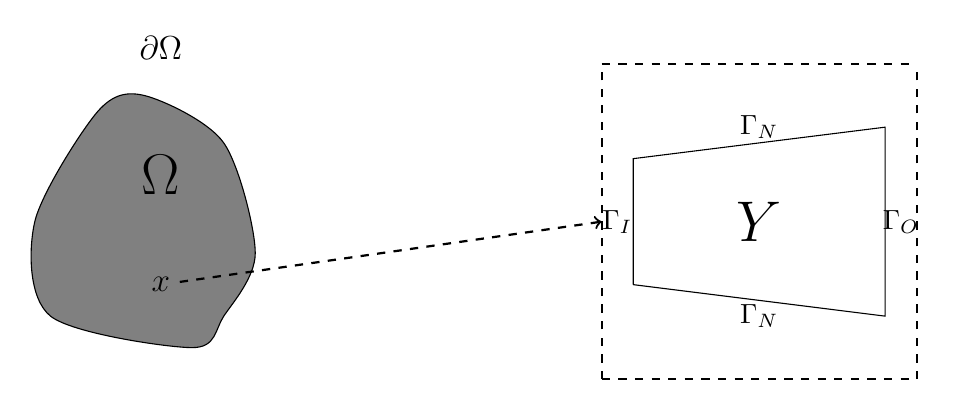
\begin{tikzpicture}[scale=0.4]
    \def\l{10};
    \def\r{1};
    \draw[black,fill=gray] plot [smooth cycle] coordinates {(\r*8, \r*2) (\r*9, \r*4) (\r*8, \r*7.5) (\r*5.5, \r*9) (\r*4, \r*8.5) (\r*2, \r*5)  (\r*2.5, \r*2) (\r*7, \r*1)};
    \node at (0.6*\l,0.45*\l + 2) (macro) {\huge $\Omega$};
    \node at (0.6*\l,0.30*\l+7.5) (macroboundary) {\large $\partial \Omega$};

    \draw [dashed, thick, step=\l] (2*\l,0) grid (3*\l,\l);
    \draw[black] (2.1*\l,0.3*\l) --(2.9*\l,0.2*\l) -- (2.9*\l,0.8*\l) -- (2.1*\l,0.7*\l) -- (2.1*\l,0.3*\l);
    \node at (2.95*\l,0.5*\l) (robin) {$\Gamma_O$};
    \node at (2.5*\l,0.20*\l) (neumann) {$\Gamma_N$};
    \node at (2.5*\l,0.80*\l) (neumann) {$\Gamma_N$};
    \node at (2.05*\l,0.50*\l) (neumann) {$\Gamma_I$};
    \node at (2.5*\l,0.5*\l) (micro) {\huge $Y$};
    \node at (\l*0.6, 0.3*\l) (x) {\large $x$};
    \draw[->, thick,dashed] (x) -- (2.0*\l, 0.5*\l);
\end{tikzpicture}   \centering
    \caption{Schematic representation of the multiscale domain}%
    \label{fig:schema}
\end{figure}


Let $u, w : \Omega \to \R$ and $v:\Omega \times Y_x \to \R$ be a triplet of functions $(u,v,w)$ that satisfies the following system of equations.
\begin{align}
    - \Delta u = - \int_{\Gamma_I} \kappa_1 u - \kappa_2 v d\sigma_y &\mbox{ in } \Omega\\
    u = u_0 &\mbox{ on } \partial\Omega_D\\
    \nabla u\cdot n_\Omega = 0 &\mbox{ on } \partial\Omega_N\\[2.5ex]
    -D_1 \Delta w = \int_{\Gamma_0} \kappa_3v - \kappa_4w d\sigma_y &\mbox{ in } \Omega\\
    \nabla w \cdot n_\Omega = 0 &\mbox { on } \partial\Omega\\[2.5ex]
    -D_2 \Delta v = 0 &\mbox{ in } \Omega \times Y_x\\
    \nabla_y v \cdot n_{Y_x} = \begin{cases}
        \kappa_1u - \kappa_2v &\mbox{ on } \Gamma_I\\
        \kappa_3v - \kappa_4w &\mbox{ on } \Gamma_O\\
        0 &\mbox{ on } \Gamma_N
    \end{cases}
\end{align}
\label{sec:future}
\subsection{Parallellisation}

Secondly, we want to parallelise the solver by taking advantage of the embarassingly parallel structure of the microsolvers. Since the bulk of the work is the assembly and solving of the linear system, there is a natural unit of separation that can be used to distribute the work on different independent processors.


There are two parallellisation paradigms that fit our use case: \emph{Distributed memory computing} and \emph{Shared memory computing}.
Distributed memory computing can be implemented by, for instance, OpenMPI where each core has their own memory and messages are shared between cores.
In this setup, the number of microsolvers is evenly divided over number of processors.
After every iteration step, the macroscopic functional over the microscopic function (the integral in \eqref{eq:main_macro}) are communicated to the processor containing the macroscopic solver, and after the macroscopic iteration step, the values of the macroscopic solver are communicated back to the corresponding microscopic solvers.

\ \\
Shared memory computing can be implemented using threads or a task-pool. In this case, a task corresponds to the assembly and solution of a microscopic system. Since all microscopic systems can be solved mutually indepently, they can be assembled in a pool, where free processors pick tasks from as soon as their previous assigned tasks finish. Each pool has access to the same memory so the overhead involved with copying data is low. Moreover, it has the added benefit over the previous approach that processors will not idle because certain microsystems might be solvable faster than other ones. For this reason, we continue exploring this approach.

\bibliography{lit}
\bibliographystyle{ieeetr}
\end{document}
